\chapter{肌肉力量优化} \label{chap:chap9}

人类遇到的每一个问题总有一个众所周知的解决方案——简洁、合理,但又错误。
\begin{flushright}
	——H. L. 门肯
\end{flushright}


\begin{figure}[!htb]
	\centering
	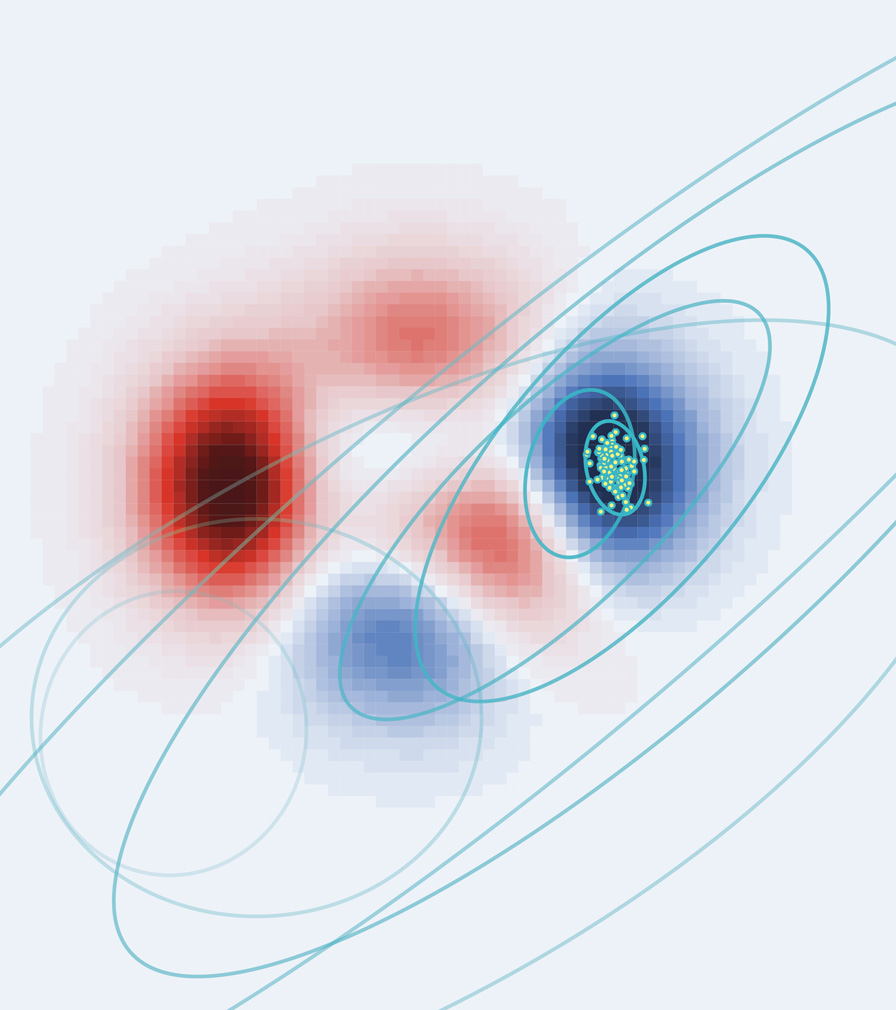
\includegraphics[width=1.0\linewidth]{chap9/9_0}
	% 加星号(*)表示不加编号
	\caption*{ \label{fig:9_0}}
\end{figure}


我一生中发现的最伟大的生物力学发现之一并非源于实验室,也未借助任何特殊设备,仅仅依靠人体不可思议的适应性。
1968年,一位名叫迪克$\cdot$福斯贝里的21岁土木工程系学生公布了他的发现,并在奥运会上以向后跳过跳高横杆的方式震惊了体育界。
一位体育记者写道:“福斯贝里跳过横杆就像一个人被人从30层楼的窗户推下去一样。”
然而,正是这种看似笨拙的跳高方式,让他创造了2.24米的奥运纪录,并最终获得金牌。


福斯贝里实际上是在高中时出于无奈才开始使用他的标志性技术。
他没能掌握当时的标准技术——“西部翻滚”,即跳高运动员面朝下越过横杆,仿佛用手臂和腿环抱横杆。
他还尝试了更古老的“剪刀”技术,即跳高运动员以近乎坐姿的姿势越过横杆,同时双腿像剪刀一样上下摆动。
但这种技术并不理想,因为跳高运动员必须将重心推到远高于横杆的高度。


在背越式跳高中,跳高运动员先向横杆一端跑去,然后向内弯曲身体,向中间跃过横杆,最后在最后一刻扭转身体,向后跃过横杆(图~\ref{fig:9_1})。
身体每次只滑过一个部位:
首先是头部和肩部,然后是躯干、臀部、膝盖,最后是双脚。
背越式跳高的一个优点是身体重心无需越过横杆。
在最高高度,臀部位于横杆上方时,背部拱起,头部和腿部悬在横杆下方,从而降低了重心。


\begin{figure}[!htb]
	\centering
	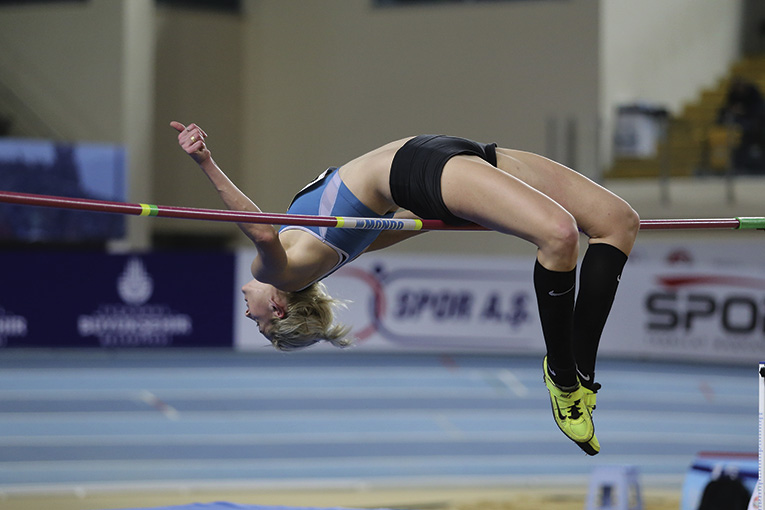
\includegraphics[width=1.0\linewidth]{chap9/9_1}
	\caption{“背越式跳高”跳高技术。
		玛雅扬$\cdot$弗曼-沙哈夫的照片,摄影:埃夫伦$\cdot$卡林巴卡克。 \label{fig:9_1}}
\end{figure}


尽管福斯贝里在发明背越式跳高时并未接受过任何正规的生物力学训练,但我们现在已经赶上了他开创性的天才。
如今,教练们使用高速录像来指导跳高运动员脚部着地的位置、蹬地前蹲到多低等等。
他们想到了福斯贝里从未想过的改进。
起跳时抬起手臂可以增加垂直动能。
臀部越过横杆后收下巴有助于迫使臀部下沉,并根据牛顿第三运动定律,将双脚抬起并越过横杆。


自1980年以来,所有跳高世界纪录都是用背越式跳高创造的,其他所有技术都已从世界舞台上消失。
现在争论的焦点是哪种背越式跳高最好:
“速度背越式”还是“力量背越式”?


对我来说,福斯贝里跳马的故事教会了我几个宝贵的教训。
首先,我们永远不应该想当然地认为流行的做事方式就是唯一或最佳方式。
但一个不那么哲学、更偏向生物力学的信息是,我们的身体拥有关节骨骼和数百块肌肉,赋予我们完成任务的无限可能,无论是像端咖啡这样看似简单的动作,还是像跳两米高这样复杂的动作。
每一个动作都需要我们的大脑协调肌肉活动。
下巴的一个简单的动作就能对我们的双脚产生影响。


为了完成任何动作,我们的身体都会解决一个优化问题,试图用最小的努力获得最大的效果。
但有一个问题,无论是数学模型还是现实世界的运动员,都可能遇到难题:局部最优并不总是全局最优。
在背越式跳高之前的运动员们都认为他们找到了最佳技术。他们错了。
但他们无法仅仅通过对西方的滚翻技术进行小幅(“局部”)调整来提高标准。
他们需要一位愿意进行大规模(“全局”)调整的运动员工程师,来改变我们对跳高应该是什么样子的理解。


在本章中,我们将探讨两种使用数值优化计算肌肉力量的广泛场景。
第一种场景出现在我们希望估算产生可观测运动的肌肉力量时。
由于人体肌肉骨骼系统存在冗余,因此通常存在许多可能的解,我们将应用优化方法,找到符合某些标准的最佳肌肉力量集。
我们将这个问题称为肌肉冗余问题(也称为肌肉力量共享问题)。
第二种场景出现在研究肌肉协调性以优化特定任务(例如跳高)的表现时。
在这种情况下,我们需要计算肌肉力量以及完成任务的身体节段运动。
如果为优化器提供跳高比赛规则和足够逼真的肌肉骨骼系统模型,它就能发现背越式跳高(以及其他我们可能从未见过的技术)。
需要注意的是,使用优化方法估算肌肉力量不仅仅是为了计算上的便利:神经系统本身就是一种优化器。
让我们来深入了解一下细节。


\section{生物和数值优化器}

人们有意识地优化他们的日常生活。
我们会决定如何分配时间、金钱、注意力和其他有限的资源,以最大限度地平衡短期和长期的满足感,并在遵守法律和其他义务等约束的同时做到这一点。
令人惊讶的是,人类也会在潜意识中优化。
回想一下第二章,我们会自然地调整步行速度、步频和其他步态变量,以使我们的交通成本接近最低——当然,除非我们赶时间,在这种情况下我们会优先考虑速度而不是代谢成本。
在学习新任务和适应新情况时,我们也会在优化过程中,根据具体情况最大化准确性、效率、舒适度和其他性能指标的某种组合。
实验表明,我们会维持一个关于身体的“内部模型”,即潜意识地理解我们刺激肌肉的程度与由此产生的身体部位运动之间的关系。
当我们置身于新环境,例如国际空间站的微重力环境或机器人装置施加的人工力场时,我们最初会显得笨拙且效率低下,因为我们在规划和预测自身动作时使用的是一个不再精准的内部模型。
在探索新环境的过程中,我们会利用视觉和其他感官反馈来调整内部模型,提高协调性。
随着时间的推移,我们会适应新环境,并通过重新学习肌肉兴奋与运动表现之间的关系,重新获得熟练的技能。


数值优化算法使用类似的探索性或“猜测-检验”策略来寻找欠定问题的解。
我们将这些猜测称为候选解,每个候选解都为所有未知数或设计变量(例如肌肉冗余问题中的肌肉激励)提供了一个数值。
每个候选解的适用性通过评估目标函数或成本函数来确定,成本函数是量化特定设计变量值集合的可取性的表达式。
能够提供最佳目标函数值(视情况而定,最小值或最大值)的候选解被称为最优解,或者简称为优化问题的解(请注意,我们可以将我们的任务定义为始终寻求最小化目标函数;为了最大化像跳跃高度这样的量,我们只需最小化其负值即可)。
正如我们将看到的,目标函数的选择会对解以及计算它所需的工作量产生深远的影响。


最优解也会受到约束条件的影响。
在许多问题中,我们要求候选解满足某些表达式(等式或不等式),才能使其成为可行解或可接受的解。
例如,在肌肉冗余问题中,我们要求所有肌肉力均为拉伸力,并且它们产生的力矩之和等于所需的净关节力矩(例如,使用逆动力学算法计算)。
由于约束条件只能减少可行解的数量(即减小解空间的大小),因此,受约束优化问题的解的目标函数值并不比优化问题不受约束时更好。
添加约束会减少您的选择。
如果约束条件过多,解空间可能为空(问题可能没有可行解)。
根据研究问题的不同,可以将一个或多个严格约束转换为软约束,这些软约束以“惩罚”的形式添加到目标函数中。
惩罚项通常通过加权因子进行缩放,以便根据其相对重要性调整它们对目标函数的贡献。
通用优化问题可以表述如下:













